\phantomsection
\chapter*{Introduzione}
\markboth{INTRODUZIONE}{}
\addcontentsline{toc}{chapter}{Introduzione}

Negli ultimi decenni, le intelligenze artificiali si sono fatte sempre più spazio nella nostra vita di tutti i giorni. Grazie ai nostri smartphone, usiamo modelli di machine learning ultra efficienti che indirizzano le nostre ricerche nella rete, e grazie a tali modelli le aziende possono mostrarci inserzioni sempre più aderenti ai nostri gusti personali. Ma il mondo dell'intelligenza artificiale ha anche importanti e utili applicazioni anche nella salvaguardia del benessere dell'individuo, ad esempio in contesti come il riconoscimento delle malattie o l'interpretazione del linguaggio parlato.

\paragraph{Human State Monitoring} Uno di questi contesti è lo \textit{Human State Monitoring}. Con questo termine si indica l'obiettivo di un sistema di raccogliere dati riguardanti l'attuale stato psico-fisico di un individuo e trarre conclusioni sulla sua condizione attuale, ad esempio interpretando un battito cardiaco elevato insieme ad un alto livello di sudorazione come uno stato di stress, o determinati movimenti facciali come una condizione di sonnolenza. L'avere a disposizione metodi efficienti di catalogare queste condizioni umane può portare a sistemi responsivi e adattivi, che modificano le proprie interfacce o i propri comportamenti accomodando lo stato psico-fisico attuale dell'utente.\\\\
Un esempio di questa applicazione lo si può trovare nel progetto europeo\\TEACHING$^{\cite{teaching2020}}$, che mira alla produzione di un toolkit per costruire applicazioni autonome efficienti che facciano uso di intelligenza simile a quella umana. L'obiettivo di questo toolkit è supportare lo sviluppo e il rilascio di applicazioni che possano sfruttare il feedback umano per ottimizzare, personalizzare e guidare il modo in cui esse forniscono i propri servizi. In altre parole, applicazioni che sfruttino lo \textit{Human State Monitoring} per adattarsi dinamicamente alle condizioni dell'utente in tempo reale.\\
Per poter realizzare questo continuo adattamento è necessario, oltre al flusso di dati in tempo reale sullo stato corrente dell'utente, anche un sistema che sappia efficientemente e correttamente interpretare questi dati e trarre conclusioni sulle attuali condizioni della persona. Questa situazione rispetta le classiche caratteristiche necessarie all'applicazione del machine learning: abbiamo dati raccolti da sensori che possono essere difettosi, per cui i dati possono contenere incertezze o essere rumorosi o incompleti, ed essendo in esame lo stato umano è molto difficile, se non impossibile, formalizzare attraverso una serie di formule la classificazione di questi dati in categorie comportamentali come affaticamento o sonnolenza.

% breve introduzione al mondo dell'addestramento machine learning per introdurre i concetti fondamentali per la tesi
\paragraph{Addestramento} L'addestramento supervisionato di un modello di machine learning avviene attraverso l'utilizzo di un insieme di dati chiamato \textit{training set}. Questo insieme contiene dati a cui è stata assegnata un'etichetta, e si contrappone all'apprendimento non supervisionato dove ai dati di addestramento non è assegnata alcuna etichetta. Nel nostro caso, prenderemo in considerazione l'apprendimento supervisionato.\\
Il modello di machine learning, attraverso una serie di algoritmi, elabora questi dati e le loro etichette cercando di apprendere quali etichette sono assegnate a quali dati. Per verificare l'apprendimento, si sottopone al modello addestrato dei dati non etichettati, denominati \textit{test set}, e si verificano le etichette che il modello assegna a tali dati controllando se ha classificato correttamente o meno. La percentuale di classificazioni corrette è chiamata \textbf{accuratezza} del modello.

\paragraph{Loss} Per misurare l'andamento dell'apprendimento di un modello di machine learning, vengono usate funzioni che vanno a valutare il modello in base alle risposte che fornisce sui dati etichettati, confrontandole con le etichette vere. Queste funzioni prendono il nome di funzioni di \textit{loss}, e ne esistono di diversi tipi a seconda del problema in esame: ad esempio, nei problemi dove ad ogni input va assegnata una risposta si/no (classificazione binaria) una loss molto usata è la cross-entropia binaria (\textit{binary crossentropy}).

\paragraph{Reti Neurali} In letteratura vengono studiati moltissimi modelli di machine learning. Si va dai più semplici come i modelli lineari, nei quali abbiamo un'equazione nella forma $y = w_0x + w_1$ e dobbiamo apprendere i $w_0$ e $w_1$ che ai dati $x$ fanno corrispondere le corrette etichette $y$, alle \textit{Support Vector Machine}, che cercano di trovare dei confini di divisione fra insiemi di dati in modo da classificarli.\\
Un'ampia area di modelli di machine learning è quella delle cosiddette \textbf{reti neurali}, studiate sin dagli anni '40. Esse prendono liberamente spunto dalla struttura dei neuroni del cervello umano (Figura \ref{fig:neurone}), che sono stati schematizzati in strutture matematiche denominate \textbf{perceptron}.
\begin{figure}[h]
	\begin{center}
		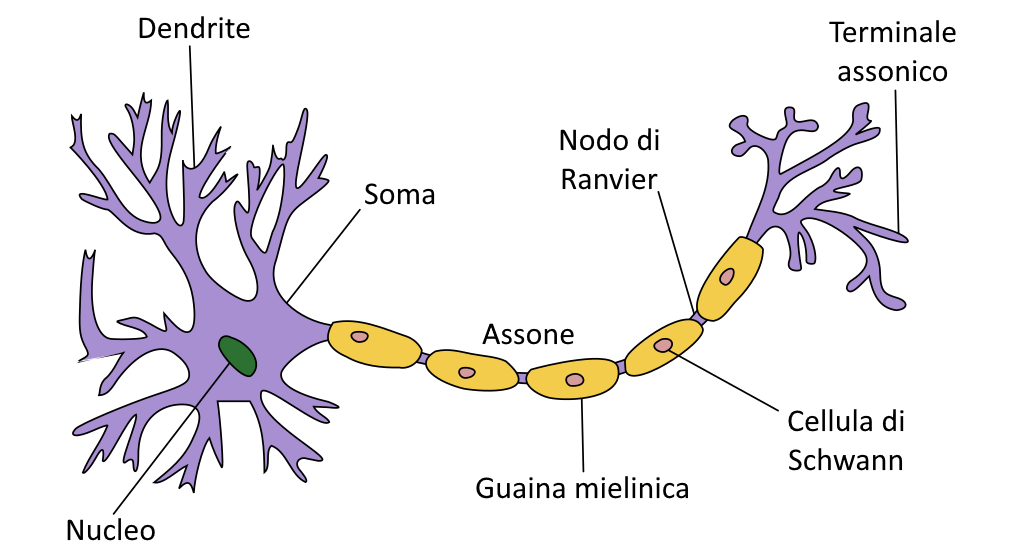
\includegraphics[width=0.75\textwidth]{img/neurone.png}
		\caption{Neurone (credits: Quasar, Wikipedia)}
		\label{fig:neurone}
	\end{center}
\end{figure}
In un perceptron (Figura \ref{fig:perceptron}), ad ogni input $x_i$ è assegnato un peso $w_i$ che lo rende più o meno importante nel contribuire al risultato $y$, che viene calcolato dal nodo attraverso la \textbf{funzione di attivazione}.\\\\
\begin{figure}[h]
	\begin{center}
		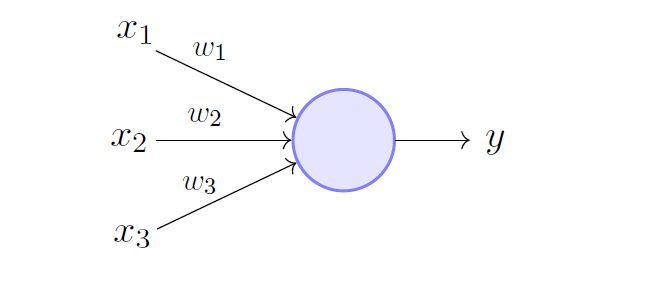
\includegraphics[width=0.5\textwidth]{img/perceptron.png}
		\caption{Perceptron}
		\label{fig:perceptron}
	\end{center}
\end{figure}
Una rete neurale (Figura \ref{fig:reteneurale}) è composta da un insieme di perceptron collegati fra loro suddivisi su livelli, o \textit{layer}: una rete neurale composta da un elevato numero di layer è detta profonda, o \textit{deep neural network}, e i layer interni sono detti layer nascosti.
\begin{figure}[b]
	\begin{center}
		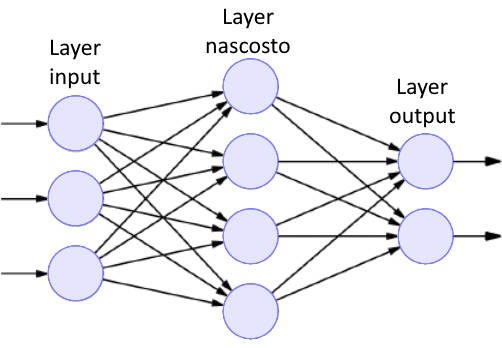
\includegraphics[width=0.75\textwidth]{img/reteneurale.jpg}
		\caption{Esempio di rete neurale}
		\label{fig:reteneurale}
	\end{center}
\end{figure}
\\\\
Le funzioni di attivazione possono essere funzioni di qualsiasi tipo, ma le più usate e studiate sono funzioni specifiche come ReLU e softmax. La funzione ReLU (\textit{Rectified Linear Unit}) è molto semplice e veloce da calcolare: restituisce la parte positiva del proprio input, e consente un migliore apprendimento nelle reti neurali profonde$^{\cite{pmlr-v15-glorot11a}}$.
\begin{equation}\label{eq:fun_relu}
ReLU(x) = max(0, x)
\end{equation}
La funzione softmax, invece, prende in input un vettore di $k$ valori e lo comprime in un vettore sempre di $k$ valori ma compresi in un intervallo $(0, 1)$ e la cui somma è 1. Vengono usate nel layer finale delle reti neurali classificatrici: ogni valore $i$  è interpretabile come la probabilità che l'input appartenga a tale classe fra le $k$ possibili.
\begin{equation}\label{eq:fun_softmax}
\sigma(\textbf{z})_j = \frac{e^{z_j}}{\sum_{k=1}^K e^{z_k}}\:\:\:\:per\:\:j = 1,\ldots,K
\end{equation}
Le funzioni di attivazione descrivono quindi il comportamento dei nodi di una rete neurale e la scelta della funzione di attivazione è un elemento importante nella strutturazione di una rete neurale. Abbiamo fatto l'esempio di ReLU, tipicamente usata nei layer nascosti, e di softmax, usata nei layer di output, ma ce ne sono molte altre adatte per altri problemi.
\paragraph{Tipologie} La struttura interna di una rete neurale influenza particolarmente i risultati che essa può ottenere. A seconda del problema che si vuole risolvere, si può avere bisogno di reti neurali con strutture interne complesse per ottenere risultati apprezzabili. In particolare, in letteratura attualmente alcune delle strutture più studiate sono (Figura \ref{fig:tipologiereti}):
\begin{itemize}
    \item[-] Reti Feed Forward (FF)
    \item[-] Reti Neurali Ricorrenti (RNN, Recurrent Neural Networks)
    \item[-] Auto Encoders (AE)
    \item[-] Reti Profonde Convolutive (DCN, Deep Convolutional Networks)
    \item[-] Echo State Networks (ESN)
\end{itemize}
e moltissime altre. Alcune strutture sono particolarmente usate su certe tipologie di problemi: ad esempio, le DCN hanno una struttura ispirata alla corteccia visiva animale e sono particolarmente usate nel campo del riconoscimento delle immagini e del linguaggio parlato, mentre le RNN mantengono informazioni riguardo gli input precedenti e consentono di modellare i comportamenti dinamici e ricorrenti delle sequenze temporali.
\begin{figure}[b]
	\begin{center}
		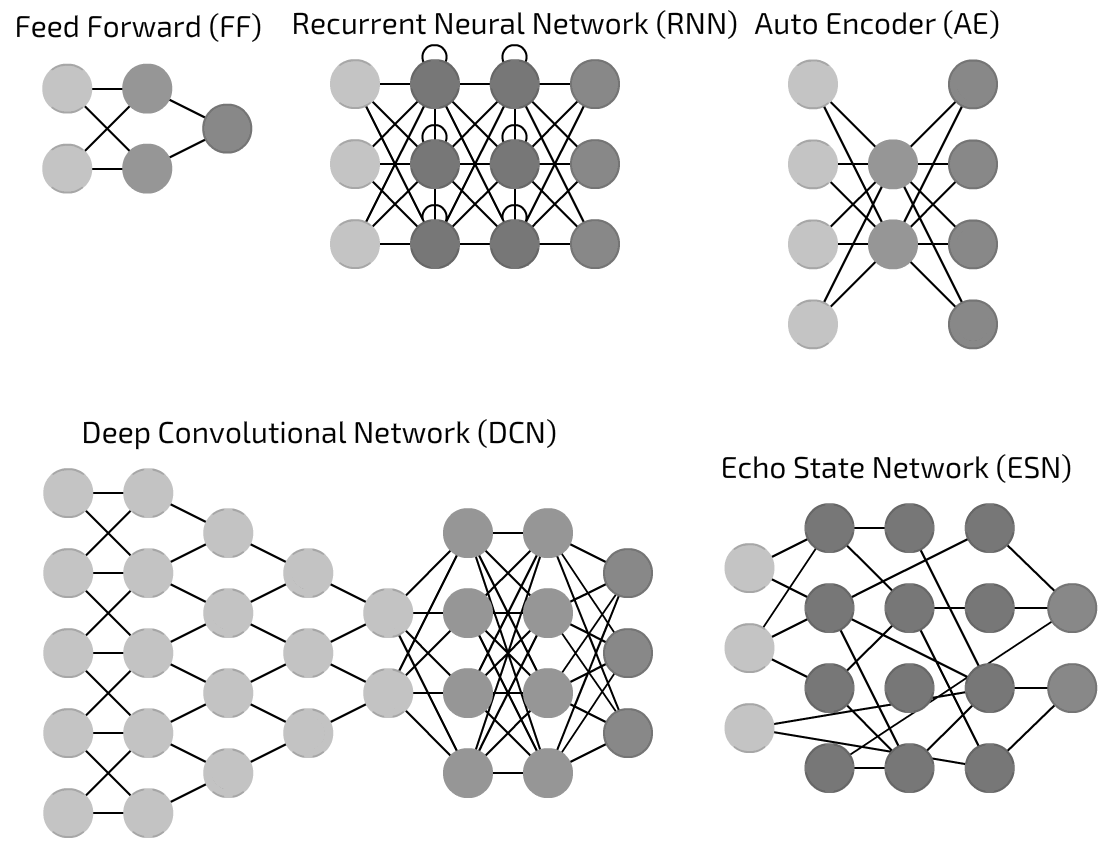
\includegraphics[width=0.95\textwidth]{img/tipologiereti.png}
		\caption{Esempi di reti neurali}
		\label{fig:tipologiereti}
	\end{center}
\end{figure}

\paragraph{Backpropagation} La retropropagazione dell'errore, \textit{backward propagation of errors}, è l'algoritmo più diffuso per l'addestramento supervisionato delle reti neurali. Questo algoritmo consiste di due fasi:
\begin{itemize}
    \item[-] \textit{Forward phase}, dove gli input vengono elaborati dalla rete neurale fino a produrre un output
    \item[-] \textit{Backward phase}, dove l'output prodotto è confrontato con l'etichetta assegnata e attraverso calcoli differenziali vengono individuati i contributi all'errore di ogni nodo. Con questi contributi, attraverso un algoritmo di ottimizzazione (solitamente, la discesa di gradiente), vengono modificati i pesi delle connessione fra i nodi, partendo dai nodi output e risalendo la rete fino ai nodi input.
\end{itemize}
Questo algoritmo richiede quindi che le funzioni di attivazione dei nodi siano differenziabili, e può soffrire di un problema che prende il nome di \textit{vanishing/exploding gradient problem}, o problema della scomparsa/esplosione del gradiente. Nel dettaglio, attraverso questo algoritmo ogni parametro del modello viene modificato, durante la \textit{backward phase}, in maniera proporzionale alla derivata parziale della funzione \textit{loss} rispetto al parametro stesso. Propagando all'indietro attraverso la regola della catena$^{(\ref{eq:catena})}$ dei gradienti compresi nell'intervallo $[0, 1]$, come nel caso di alcune funzioni di attivazione, il prodotto diventa tanto più piccolo quanto più è profonda la rete neurale o, viceversa, esplodere in caso di gradienti dai valori elevati.
\begin{equation}\label{eq:catena}
D\left[f(g(x))\right] = f'(g(x))\cdot g'(x)
\end{equation}
Questo problema viene mitigato dall'uso di funzioni di attivazioni diverse, come le già citate ReLU$^{(\ref{eq:fun_relu})}$ e softmax$^{(\ref{eq:fun_softmax})}$, o dall'uso di algoritmi di addestramento che fanno uso solo del segno del gradiente e non della sua norma, come l'algoritmo Rprop$^{\cite{Riedmiller92rprop-}}$.\\
Nelle reti neurali ricorrenti, un grande contributo alla mitigazione del problema è avvenuto grazie all'introduzione delle LSTM, \textit{Long-Short Term Memory}, che mantengono informazioni sullo stato del modello senza propagarle attraverso funzioni non lineari.

\paragraph{Continual Learning} L'addestramento di un modello di machine learning attraverso un \textit{training set} disponibile fin da subito e fornito al modello tutto in una volta è denominato "addestramento \textit{offline}", o \textit{offline training}. Esistono contesti, però, dove i dati necessari o utili all'addestramento non sono subito tutti disponibili, ma diventano tali col passare del tempo. Un esempio di questa situazione sono i sistemi di raccomandazione in servizi come Netflix o YouTube: essi imparano continuamente i gusti dell'utente, in modo da fornire suggerimenti su video e film sempre adatti ai gusti del momento. Questa situazione, in cui i dati di addestramento diventano disponibili col passare del tempo e cioè di addestramento continuativo, è detta "addestramento \textit{continual}", o \textit{continual learning}.\\
Nel caso del \textit{continual learning}, un grosso ostacolo è quello denominato \textit{catastrophic forgetting}$^{\cite{MCCLOSKEY1989109}}$: quando una rete neurale già addestrata viene addestrata su nuovi dati, essa tenderà a dimenticare ciò che ha appreso sui dati precedenti. Questa situazione è una manifestazione del cosiddetto dilemma della \textbf{plasticità-stabilità}: si ha stabilità quando la nuova conoscenza non interferisce con la vecchia conoscenza, mentre la plasticità è ottenuta quando la nuova conoscenza migliora la conoscenza precedente e viceversa. Questi due obiettivi sono in contrapposizione fra loro e mantenere un buon compromesso fra i due è uno degli obiettivi chiave degli algoritmi e attuale campo di studio.\\\\
Il continual learning si rende ancora più necessario in un mondo in continua e rapida evoluzione, e apporta al machine learning un cambiamento di paradigma al pari dell'introduzione della filosofia Agile$^{\cite{agilemanifesto}}$ nel mondo dell'ingegneria del software: mentre in molti dei modelli di machine learning correnti l'addestramento è eseguito da zero e il modello viene utilizzato così com'è, con un procedimento al pari dei primi approcci "a cascata" allo sviluppo software, il continual learning fornisce a questo mondo la possibilità di produrre modelli che vengono migliorati iterativamente ogni volta che c'è bisogno senza dover addestrare un nuovo modello da zero. "Il parallelismo sta nell'equiparare i dati ai requisiti (arrivano in maniera continuativa e cambiano nel tempo) e l'addestramento alla fase di design e sviluppo, che porta al prodotto software (che nel nostro caso è la funzione di predizione realizzata dal modello di machine learning)."$^{\cite{lomonaco_2019}}$

\paragraph{Conclusione} Lo \textit{human state monitoring} è un ambiente sempre più utile e importante nella realizzazione di sistemi personalizzati che rispondono dinamicamente allo stato attuale dell'utente: un esempio può essere la riduzione della velocità di un veicolo a guida autonoma quando l'utente alla guida è in stato di sonnolenza, e quindi poco attento agli eventuali errori del veicolo.\\
Per realizzare questi modelli di machine learning si rendono necessarie reti neurali ricorrenti, poiché abbiamo a che fare con flussi di dati temporali raccolti da vari sensori posti sull'utente, che devono adattarsi in maniera continuativa all'utente attuale (nell'esempio, il proprietario del veicolo) avvalendosi quindi di tecniche di continual learning, che non soffrano del \textit{catastrophic forgetting}.\\
Si necessitano quindi di metriche per misurare nel tempo l'efficienza e la precisione di questi modelli sottoposti a continual learning, per giudicare l'applicabilità delle tecniche in esame applicate allo \textit{human state monitoring}.